\let\negmedspace\undefined
\let\negthickspace\undefined
\documentclass[journal]{IEEEtran}
\usepackage[a5paper, margin=10mm, onecolumn]{geometry}

\setlength{\headheight}{1cm} 
\setlength{\headsep}{0mm}     

\usepackage{gvv-book}
\usepackage{gvv}
\usepackage{cite}
\usepackage{amsmath,amssymb,amsfonts,amsthm}
\usepackage{algorithmic}
\usepackage{graphicx}
\usepackage{textcomp}
\usepackage{xcolor}
\usepackage{txfonts}
\usepackage{listings}
\usepackage{enumitem}
\usepackage{mathtools}
\usepackage{gensymb}
\usepackage{comment}
\usepackage[breaklinks=true]{hyperref}
\usepackage{tkz-euclide} 
\usepackage[latin1]{inputenc}                                
\usepackage{color}                                            
\usepackage{array}                                            
\usepackage{longtable}                                       
\usepackage{calc}                                             
\usepackage{multirow}                                         
\usepackage{hhline}                                           
\usepackage{ifthen}                                           
\usepackage{lscape}
\begin{document}

\bibliographystyle{IEEEtran}
\vspace{3cm}

\title{4.13.88}
\author{AI25BTECH11019 - MENAVATH SAI SANJANA}
{\let\newpage\relax\maketitle}

\renewcommand{\thefigure}{\theenumi}
\renewcommand{\thetable}{\theenumi}
\setlength{\intextsep}{10pt} 

\numberwithin{equation}{enumi}
\numberwithin{figure}{enumi}
\renewcommand{\thetable}{\theenumi}

\textbf{Question}:\\
A line with positive direction cosines passes through the point 
$P(2,-1,2)$ and makes equal angles with the coordinate axes.  
The line meets the plane $2x+y+z=9$ at point $Q$.  
Find the length of $PQ$.  
\\
\bigskip
\textbf{Solution: }

\begin{align}
\text{Let } \vec{P} &= \myvec{2\\-1\\2}, \quad \vec{d} = \myvec{1\\1\\1}, \\
\vec{r} &= \vec{P} + t\vec{d} = \myvec{2+t\\-1+t\\2+t}.
\end{align}

Plane equation in vector form:
\begin{align}
\vec{n}^T \vec{r} = 9, \quad \vec{n} = \myvec{2\\1\\1}.
\end{align}

Intersection point:
\begin{align}
\vec{n}^T (\vec{P} + t \vec{d}) &= 9,\\
\myvec{2 & 1 & 1} \, (\myvec{2\\-1\\2} + t \myvec{1\\1\\1}) &= 9,\\
\\
5 + 4t &= 9 \;\Rightarrow\; t = 1.
\end{align}

Coordinates of Q:
\begin{align}
\vec{Q} &= \vec{P} + t \vec{d} = \myvec{2\\-1\\2} + 1 \cdot \myvec{1\\1\\1} = \myvec{3\\0\\3}.
\end{align}

Vector PQ and its magnitude:
\begin{align}
\vec{PQ} &= \vec{Q} - \vec{P} = \myvec{3\\0\\3} - \myvec{2\\-1\\2} = \myvec{1\\1\\1},\\
|\vec{PQ}| &= \sqrt{\vec{PQ}^T \vec{PQ}} = \sqrt{1^2 + 1^2 + 1^2} = \sqrt{3}.
\end{align}

\vspace{1cm}

\noindent\textbf{Conclusion:}  
The vector and length of $PQ$ are
\begin{align}
\vec{PQ} &= \myvec{1\\1\\1},\\
|PQ| &= \sqrt{3}.
\end{align}

\begin{figure}[ht!]
    \centering
    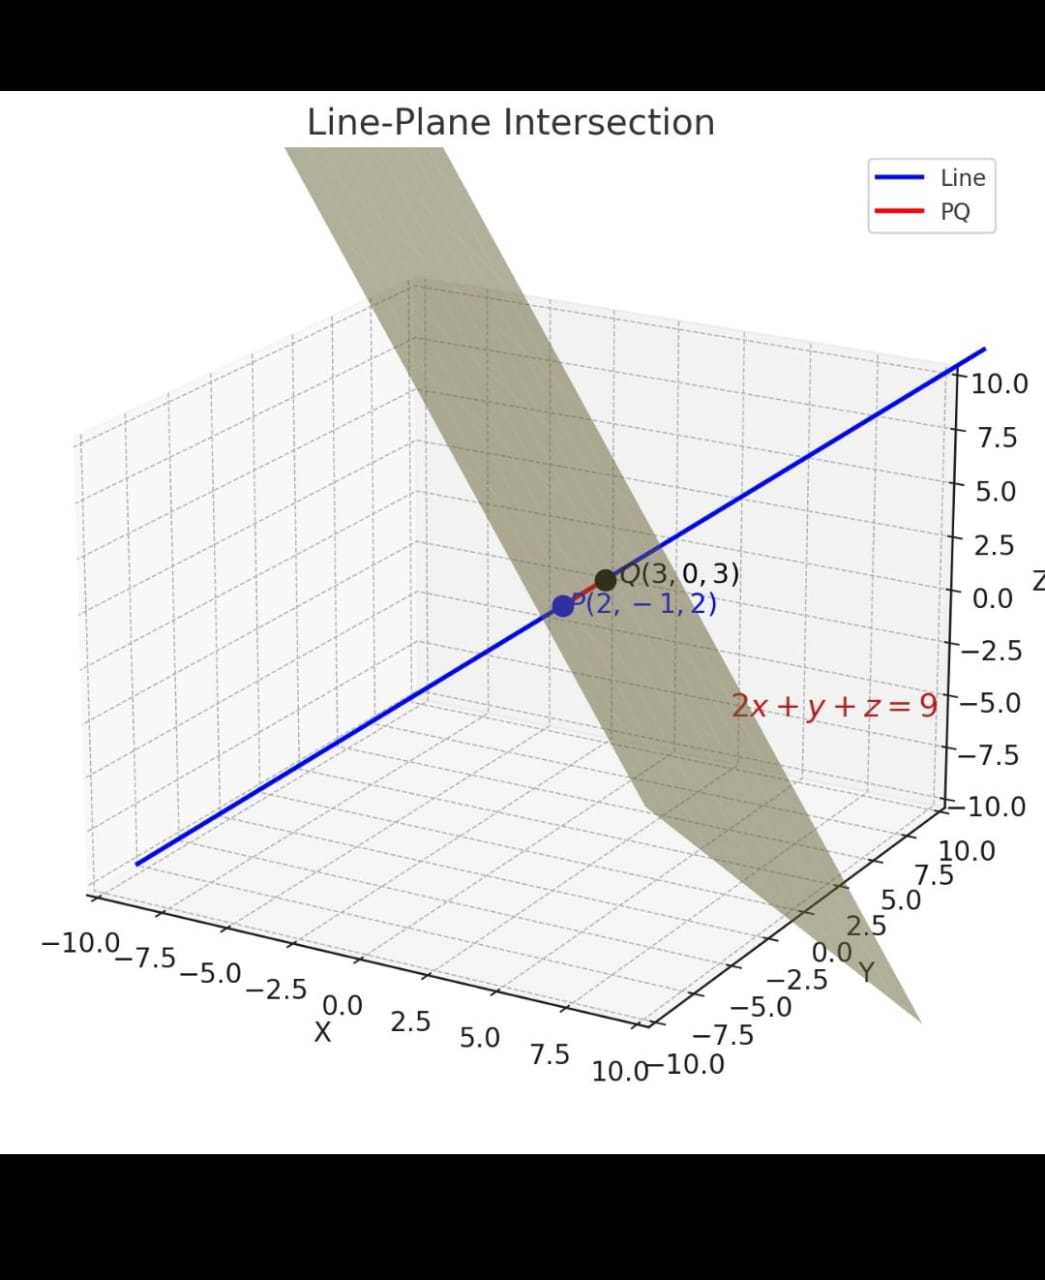
\includegraphics[width=0.8\textwidth]{figs/matgeo-4.13.88.jpeg}
    \caption{}
    \label{fig:matgeo-4.13.88}
\end{figure}

\end{document}

